\PassOptionsToPackage{unicode=true}{hyperref} % options for packages loaded elsewhere
\PassOptionsToPackage{hyphens}{url}
%
\documentclass[]{book}
\usepackage{lmodern}
\usepackage{amssymb,amsmath}
\usepackage{ifxetex,ifluatex}
\usepackage{fixltx2e} % provides \textsubscript
\ifnum 0\ifxetex 1\fi\ifluatex 1\fi=0 % if pdftex
  \usepackage[T1]{fontenc}
  \usepackage[utf8]{inputenc}
  \usepackage{textcomp} % provides euro and other symbols
\else % if luatex or xelatex
  \usepackage{unicode-math}
  \defaultfontfeatures{Ligatures=TeX,Scale=MatchLowercase}
\fi
% use upquote if available, for straight quotes in verbatim environments
\IfFileExists{upquote.sty}{\usepackage{upquote}}{}
% use microtype if available
\IfFileExists{microtype.sty}{%
\usepackage[]{microtype}
\UseMicrotypeSet[protrusion]{basicmath} % disable protrusion for tt fonts
}{}
\IfFileExists{parskip.sty}{%
\usepackage{parskip}
}{% else
\setlength{\parindent}{0pt}
\setlength{\parskip}{6pt plus 2pt minus 1pt}
}
\usepackage{hyperref}
\hypersetup{
            pdftitle={Time Series Analysis and Forecasting with ADAM},
            pdfauthor={Ivan Svetunkov},
            pdfborder={0 0 0},
            breaklinks=true}
\urlstyle{same}  % don't use monospace font for urls
\usepackage{color}
\usepackage{fancyvrb}
\newcommand{\VerbBar}{|}
\newcommand{\VERB}{\Verb[commandchars=\\\{\}]}
\DefineVerbatimEnvironment{Highlighting}{Verbatim}{commandchars=\\\{\}}
% Add ',fontsize=\small' for more characters per line
\usepackage{framed}
\definecolor{shadecolor}{RGB}{248,248,248}
\newenvironment{Shaded}{\begin{snugshade}}{\end{snugshade}}
\newcommand{\AlertTok}[1]{\textcolor[rgb]{0.94,0.16,0.16}{#1}}
\newcommand{\AnnotationTok}[1]{\textcolor[rgb]{0.56,0.35,0.01}{\textbf{\textit{#1}}}}
\newcommand{\AttributeTok}[1]{\textcolor[rgb]{0.77,0.63,0.00}{#1}}
\newcommand{\BaseNTok}[1]{\textcolor[rgb]{0.00,0.00,0.81}{#1}}
\newcommand{\BuiltInTok}[1]{#1}
\newcommand{\CharTok}[1]{\textcolor[rgb]{0.31,0.60,0.02}{#1}}
\newcommand{\CommentTok}[1]{\textcolor[rgb]{0.56,0.35,0.01}{\textit{#1}}}
\newcommand{\CommentVarTok}[1]{\textcolor[rgb]{0.56,0.35,0.01}{\textbf{\textit{#1}}}}
\newcommand{\ConstantTok}[1]{\textcolor[rgb]{0.00,0.00,0.00}{#1}}
\newcommand{\ControlFlowTok}[1]{\textcolor[rgb]{0.13,0.29,0.53}{\textbf{#1}}}
\newcommand{\DataTypeTok}[1]{\textcolor[rgb]{0.13,0.29,0.53}{#1}}
\newcommand{\DecValTok}[1]{\textcolor[rgb]{0.00,0.00,0.81}{#1}}
\newcommand{\DocumentationTok}[1]{\textcolor[rgb]{0.56,0.35,0.01}{\textbf{\textit{#1}}}}
\newcommand{\ErrorTok}[1]{\textcolor[rgb]{0.64,0.00,0.00}{\textbf{#1}}}
\newcommand{\ExtensionTok}[1]{#1}
\newcommand{\FloatTok}[1]{\textcolor[rgb]{0.00,0.00,0.81}{#1}}
\newcommand{\FunctionTok}[1]{\textcolor[rgb]{0.00,0.00,0.00}{#1}}
\newcommand{\ImportTok}[1]{#1}
\newcommand{\InformationTok}[1]{\textcolor[rgb]{0.56,0.35,0.01}{\textbf{\textit{#1}}}}
\newcommand{\KeywordTok}[1]{\textcolor[rgb]{0.13,0.29,0.53}{\textbf{#1}}}
\newcommand{\NormalTok}[1]{#1}
\newcommand{\OperatorTok}[1]{\textcolor[rgb]{0.81,0.36,0.00}{\textbf{#1}}}
\newcommand{\OtherTok}[1]{\textcolor[rgb]{0.56,0.35,0.01}{#1}}
\newcommand{\PreprocessorTok}[1]{\textcolor[rgb]{0.56,0.35,0.01}{\textit{#1}}}
\newcommand{\RegionMarkerTok}[1]{#1}
\newcommand{\SpecialCharTok}[1]{\textcolor[rgb]{0.00,0.00,0.00}{#1}}
\newcommand{\SpecialStringTok}[1]{\textcolor[rgb]{0.31,0.60,0.02}{#1}}
\newcommand{\StringTok}[1]{\textcolor[rgb]{0.31,0.60,0.02}{#1}}
\newcommand{\VariableTok}[1]{\textcolor[rgb]{0.00,0.00,0.00}{#1}}
\newcommand{\VerbatimStringTok}[1]{\textcolor[rgb]{0.31,0.60,0.02}{#1}}
\newcommand{\WarningTok}[1]{\textcolor[rgb]{0.56,0.35,0.01}{\textbf{\textit{#1}}}}
\usepackage{longtable,booktabs}
% Fix footnotes in tables (requires footnote package)
\IfFileExists{footnote.sty}{\usepackage{footnote}\makesavenoteenv{longtable}}{}
\usepackage{graphicx,grffile}
\makeatletter
\def\maxwidth{\ifdim\Gin@nat@width>\linewidth\linewidth\else\Gin@nat@width\fi}
\def\maxheight{\ifdim\Gin@nat@height>\textheight\textheight\else\Gin@nat@height\fi}
\makeatother
% Scale images if necessary, so that they will not overflow the page
% margins by default, and it is still possible to overwrite the defaults
% using explicit options in \includegraphics[width, height, ...]{}
\setkeys{Gin}{width=\maxwidth,height=\maxheight,keepaspectratio}
\setlength{\emergencystretch}{3em}  % prevent overfull lines
\providecommand{\tightlist}{%
  \setlength{\itemsep}{0pt}\setlength{\parskip}{0pt}}
\setcounter{secnumdepth}{5}
% Redefines (sub)paragraphs to behave more like sections
\ifx\paragraph\undefined\else
\let\oldparagraph\paragraph
\renewcommand{\paragraph}[1]{\oldparagraph{#1}\mbox{}}
\fi
\ifx\subparagraph\undefined\else
\let\oldsubparagraph\subparagraph
\renewcommand{\subparagraph}[1]{\oldsubparagraph{#1}\mbox{}}
\fi

% set default figure placement to htbp
\makeatletter
\def\fps@figure{htbp}
\makeatother

\usepackage{booktabs}
\usepackage{amsthm, graphicx, mathtools, amssymb}
\makeatletter
\def\thm@space@setup{%
  \thm@preskip=8pt plus 2pt minus 4pt
  \thm@postskip=\thm@preskip
}
\makeatother

\newtheorem*{remark}{Remark}
\usepackage[]{natbib}
\bibliographystyle{apalike}

\title{Time Series Analysis and Forecasting with ADAM}
\author{Ivan Svetunkov}
\date{2020-06-23}

\begin{document}
\maketitle

{
\setcounter{tocdepth}{1}
\tableofcontents
}
\hypertarget{preface}{%
\chapter*{Preface}\label{preface}}
\addcontentsline{toc}{chapter}{Preface}

This textbook uses two packages from R, namely \texttt{greybox}, which focuses on forecasting using regression models, and \texttt{smooth}, which implements Single Source of Error (SSOE) state space models for purposes of time series analysis and forecasting. The textbook focuses on explaining how ADAM (``ADAM is Dynamic Adaptive Model'' - recursive acronym), one of the \texttt{smooth} functions (introduced in v3.0.0) works, also showing how it can be used in practice with examples from R. ADAM is a state space model based on exponential smoothing in ETS format and ARIMA. It encompasses both models and is expanded by introducing:

\begin{enumerate}
\def\labelenumi{\arabic{enumi}.}
\tightlist
\item
  Explanatory variables (including time varying parameters);
\item
  Multiple frequencies;
\item
  Handling of intermittent data (data with natural zeroes);
\item
  Handling of missing data;
\item
  Variables and components selection and combination;
\item
  Analysis of parameters of the model;
\item
  And other minor features.
\end{enumerate}

All these extentions are needed in order to solve specific real life problems, so we will have examples and case studies later in the book, in order to see how all of this can be used.

If you want to run exampels from the textbook, two packages are needed \citep{R-greybox, R-smooth}:

\begin{Shaded}
\begin{Highlighting}[]
\KeywordTok{install.packages}\NormalTok{(}\StringTok{"greybox"}\NormalTok{)}
\KeywordTok{install.packages}\NormalTok{(}\StringTok{"smooth"}\NormalTok{)}
\end{Highlighting}
\end{Shaded}

Some explanations of functions from the packages are given in my blog: \href{https://forecasting.svetunkov.ru/en/category/r-en/greybox/}{Package greybox for R}, \href{https://forecasting.svetunkov.ru/en/category/r-en/smooth/}{Package smooth for R}.

A very important thing to note is that this textbook \textbf{does not use \texttt{tidyverse} packages}. I like base R, and, to be honest, I am sure that \texttt{tidyverse} packages are great, but I have never needed them in my research. So, I will not use pipeline operators, \texttt{tibble} or \texttt{tsibble} objects and \texttt{ggplot2}. It is assumed throughout the textbook that you can do all those nice tricks on your own if you want to.

If you want to get in touch with me, there are lots of ways to do that: comments section on any page of \href{https://forecasting.svetunkov.ru/}{my website}, \href{https://ivan.svetunkov.ru/}{my Russian website}, \href{https://vk.com/isvetunkov}{vk.com}, \href{https://www.facebook.com/isvetunkov}{Facebook}, \href{https://www.linkedin.com/in/isvetunkov}{Linkedin}, \href{https://twitter.com/iSvetunkov}{Twitter}.

You can also find me on \href{https://www.researchgate.net/profile/Ivan_Svetunkov}{ResearchGate}, \href{http://stats.stackexchange.com/users/87585/ivan-svetunkov}{StackExchange} and \href{http://stackoverflow.com/users/5296618/ivan-svetunkov}{StackOverflow}, although I'm not really active there. Finally, I also have \href{https://github.com/config-i1}{GitHub} account.

\hypertarget{intro}{%
\chapter{Introduction}\label{intro}}

I have started writing this book in 2020 during the COVID-19 pandemic, having figured out that it has been more than 10 years since the publishing of the fundamental textbook of \citep{Hyndman2008b}, who discuss ETS (Error-Trend-Seasonality) framework in the Single Source of Error (SSOE) form. If you are interested in knowing more about exponential smoothing, then this is a must read material on the topic. However, there has been some progress in the area since 2008, and I have developed some models and functions based on ETS, making the framework a bit more flexible and general. Given that the publication of all the aspects of these models in peer-reviewed journals is difficult and challenging, I have decided to summarise all the progress in the book, showing what happens inside the models and how to use the functions in different cases.

Before we move to nitty gritty details of the models, it is important to agree what we are talking about. So, here is a couple of definitions:

\begin{itemize}
\tightlist
\item
  \textbf{Statistical model} (or `stochastic model', or just `model' in this textbook) is a `mathematical representation of a real phenomenon with a complete specification of distribution and parameters' \citep{Svetunkov2017a}. Very roughly, the statistical model is something that contains a structure (defined by its parameters) and a noise that follows some distribution.
\item
  \textbf{True model} is the idealistic statistical model that is correctly specified (has all the necessary components in correct form), applied to the data in population. By this definition, true model is never reachable in reality, but it is achievable in theory if for some reason we know what components and variables should definitely be in the model and have all the data in the world.
\item
  \textbf{Estimated model} (aka `used model' or `applied model') is the statistical model that was constructed and estimated on the available sample of data. This typically differs from the true model, because the latter is not known. Even if the specification of the true model is known for some reason, the parameters of the estimated model will differ from the true parameters due to sampling randomness.
\item
  \textbf{Data generating process} (DGP) is an artificial statistical model, showing how the data could be generated in theory. This notion is utopic and can be used in simulation experiments in order to check, how the selected model with the specific estimator behave in a specific setting. In real life, the data is not generated from any process, but is usually based on complex interactions between different agents in a dynamic environment. Note that I make a distinction between DGP and true model, because I do not think that the idea of something being generated using a mathematical formula is helpful. Many statisticians will not agree with me on this distinction.
\item
  \textbf{Forecasting method} is a mathematical procedure that generates point and / or interval forecasts, with or without a statistical model \citep{Svetunkov2017a}. Very roughly, forecasting method is just a way of producing forecasts that does not explain how the components of time series interact with each other. It might be needed in order to filter out the noise and extrapolate the structure.
\end{itemize}

Later in this book, we will see several examples of statistical models, forecasting methods, DGPs and other notions.

Note that this textbook assumes that the reader is familiar with introductory statistics and knows forecasting principles. \citep{Hyndman2018} can be a good start if you do not know either. We will also use elements of linear algebra to explain some modelling parts, but this will not be the main focus of the textbook and you will be able to skip the more challenging parts without jeopardising the main understanding of the topic.

\hypertarget{forecastingProcess}{%
\section{Forecasting process and forecasts evaluation}\label{forecastingProcess}}

Before we move to the discussion of models and their estimation it makes sense to discuss the forecasting process and how the forecasts should be evaluated.

\hypertarget{fixed-origin-versus-rolling-origin}{%
\subsection{Fixed origin versus rolling origin}\label{fixed-origin-versus-rolling-origin}}

\hypertarget{errorMeasures}{%
\subsection{Measuring accuracy of point forecasts}\label{errorMeasures}}

\hypertarget{measuring-uncertainty}{%
\subsection{Measuring uncertainty}\label{measuring-uncertainty}}

\hypertarget{a-short-introduction-to-main-statistical-ideas}{%
\chapter{A short introduction to main statistical ideas}\label{a-short-introduction-to-main-statistical-ideas}}

Before moving forward and discussing distributions and models, it is also quite important to make sure that we undersatnd what \textbf{bias}, \textbf{efficiency} and \textbf{consistency} of estimates of parameters mean. Although there are strict statistical definitions of the aforementioned terms (you can easily find them in Wikipedia or anywhere else), I do not want to copy-paste them here, because there are only a couple of important points worth mentioning in our context.

\textbf{Bias} refers to the expected difference between the estimated value of parameter (on a specific sample) and the ``true'' one (in the true model). Having unbiased estimates of parameters is important because they should lead to more accurate forecasts (at least in theory). For example, if the estimated parameter is equal to zero, while in fact it should be 0.5, then the model would not take the provided information into account correctly and as a result will produce less accurate point forecasts and incorrect prediction intervals. In inventory context this may mean that we constantly order 100 units less than needed only because the parameter is lower than it should be.

\textbf{Efficiency} means, if the sample size increases, then the estimated parameters will not change substantially, they will vary in a narrow range (variance of estimates will be small). In the case with inefficient estimates the increase of sample size from 50 to 51 observations may lead to the change of a parameter from 0.1 to, let's say, 10. This is bad because the values of parameters usually influence both point forecasts and prediction intervals. As a result the inventory decision may differ radically from day to day. For example, we may decide that we urgently need 1000 units of product on Monday, and order it just to realise on Tuesday that we only need 100. Obviously this is an exaggeration, but no one wants to deal with such an erratically behaving model, so we need to have efficient estimates of parameters.

\textbf{Consistency} means that our estimates of parameters will get closer to the stable values (true value in the population) with the increase of the sample size. This is important because in the opposite case estimates of parameters will diverge and become less and less realistic. This once again influences both point forecasts and prediction intervals, which will be less meaningful than they should have been. In a way consistency means that with the increase of the sample size the parameters will become more efficient and less biased. This in turn means that the more observations we have, the better.

\begin{remark}
There is a prejudice in the world of practitioners that the situation in
the market changes so fast that the old observations become useless very
fast. As a result many companies just through away the old data.
Although, in general the statement about the market changes is true, the
forecasters tend to work with the models that take this into account
(e.g.~Exponential smoothing, ARIMA, discussed in this book). These
models adapt to the potential changes. So, we may benefit from the old
data because it allows us getting more consistent estimates of
parameters. Just keep in mind, that you can always remove the annoying
bits of data but you can never un-throw away the data.
\end{remark}

Another important aspect to cover is what the term \textbf{asymptotic} means in our context. Here and after in this book, when this word is used, we refer to an unrealistic hypothetic situation of having all the data in the multiverse, where the time index \(t \rightarrow \infty\). While this is impossible, the idea is useful, because asymptotic behaviour of estimators and models is helpful on large samples of data.

Finally, we will use different estimation techniques throughout this book, one of the main of which is \textbf{Maximum Likelihood Estimate} (MLE). We will not go into explanation of what specifically this is at this stage, but a rough understanding should suffice. In case of MLE, we assume that a variable follows a parametric distribution and that the parameters of the model that we use can be optimised in order to maximise the respective probability density function. The main advantages of MLE is that it gives consistent, asymptotically efficient and normal estimates of parameters.

Now that we have a basic understanding of these statistical terms, we can move to the next topic, distributions.

\hypertarget{distributions}{%
\section{Theory of distributions}\label{distributions}}

There are several probability distributions that will be helpful in the further chapters of this textbook. Here, I want to briefly discuss those of them that will be useful.

\hypertarget{normal-distribution}{%
\subsection{Normal distribution}\label{normal-distribution}}

Every statistical textbook has normal distribution. It is that one famous bell-curved distribution that every statistician likes because it is easy to work with and it is an asymptotic distribution for many other well-behaved distributions in some conditions (so called ``Centrel Limit Theorem''). Here is the probability density function (PDF) of this distribution:
\begin{equation} \label{eq:Normal}
    f(y_t) = \frac{1}{\sqrt{2 \pi \sigma^2}} \exp \left( -\frac{\left(y_t - \mu_t \right)^2}{2 \sigma^2} \right) ,
\end{equation}
where \(y_t\) is the value of the response variable, \(\mu_t\) is the mean on observation \(t\) and \(\sigma^2\) is the variance of the error term. The maximum likelihood estimate of \(\sigma^2\) is:
\begin{equation} \label{eq:sigmaNormal}
    \hat{\sigma}^2 = \frac{1}{T} \sum_{t=1}^T \left(y_t - \mu_t \right)^2 ,
\end{equation}
which coincides with Mean Squared Error (MSE), discussed in the \protect\hyperlink{errorMeasures}{section 1}.

And here how this distribution looks:

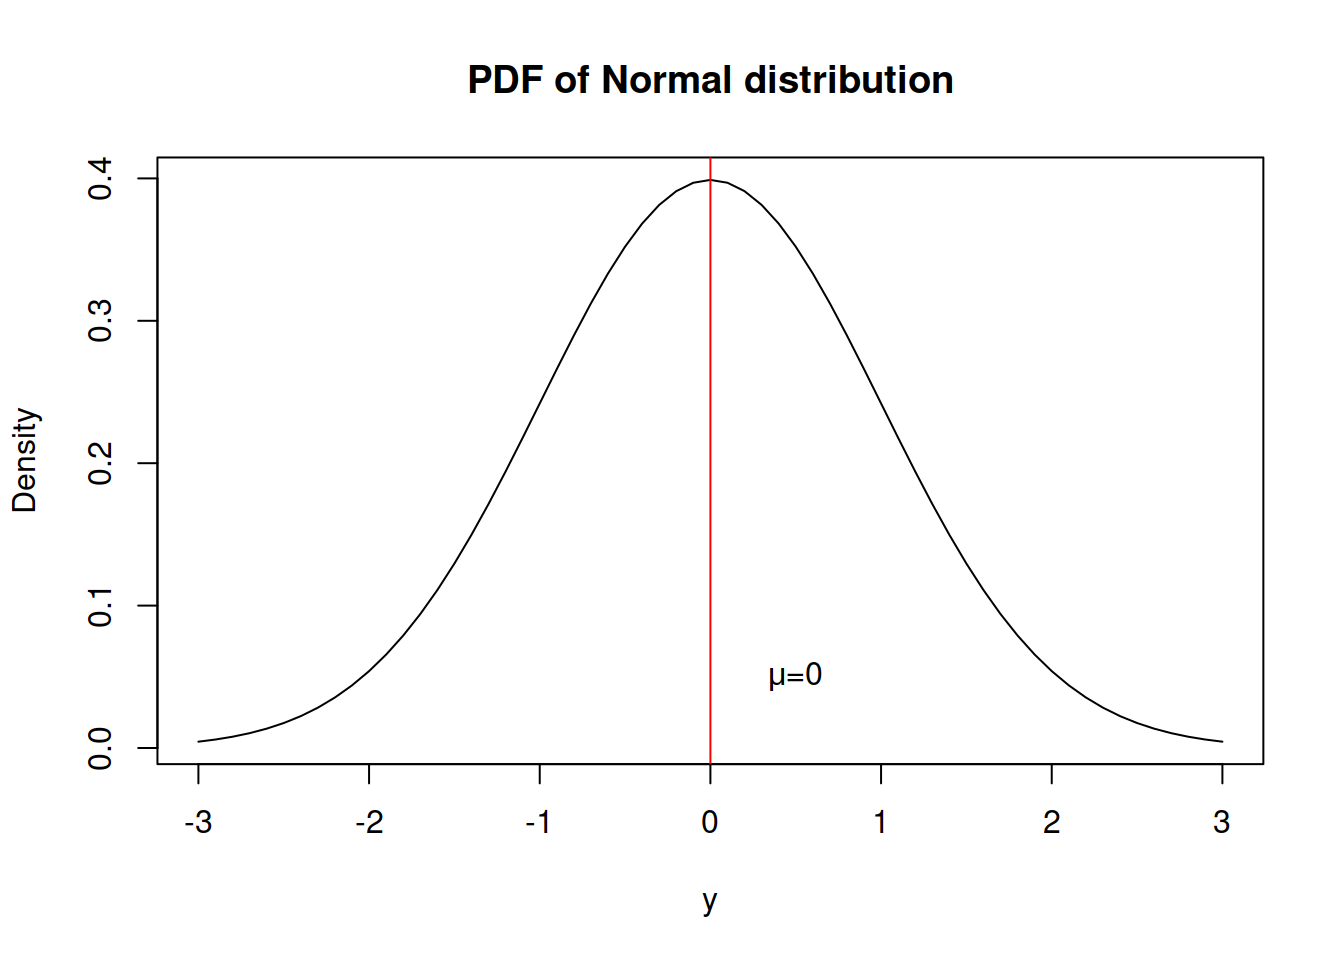
\includegraphics{adam_files/figure-latex/dnormPlot-1.pdf}

What we typically assume in the basic time series models is that a variable is random and follows normal distribution, meaning that there is a central tendency (in our case - the mean \(mu\)), around which the concentration of values is the highest and there are other potential cases, but their probabilitu of appearance reduces proportionally to the distance from the centre.

The normal distribution has skewness of zero and kurtosis of 3 (and excess kurtosis, being kurtosis minus three, of 0).

Additionally, if normal distribution is used for the maximum likelihood estimation of a model, it gives the same parameters as the minimisation of MSE would give.

\hypertarget{laplace-distribution}{%
\subsection{Laplace distribution}\label{laplace-distribution}}

A more exotic distribution is Laplace, which has some similarities with Normal, but has higher excess. It has the following PDF:

\begin{equation} \label{eq:Laplace}
    f(y_t) = \frac{1}{2 s} \exp \left( -\frac{\left| y_t - \mu_t \right|}{s} \right) ,
\end{equation}
where \(s\) is the scale parameter, which, when estimated using likelihood, is equal to the Mean Absolute Error (MAE):
\begin{equation} \label{eq:sLaplace}
    \hat{s} = \frac{1}{T} \sum_{t=1}^T \left| y_t - \mu_t \right| .
\end{equation}

It has the following shape:

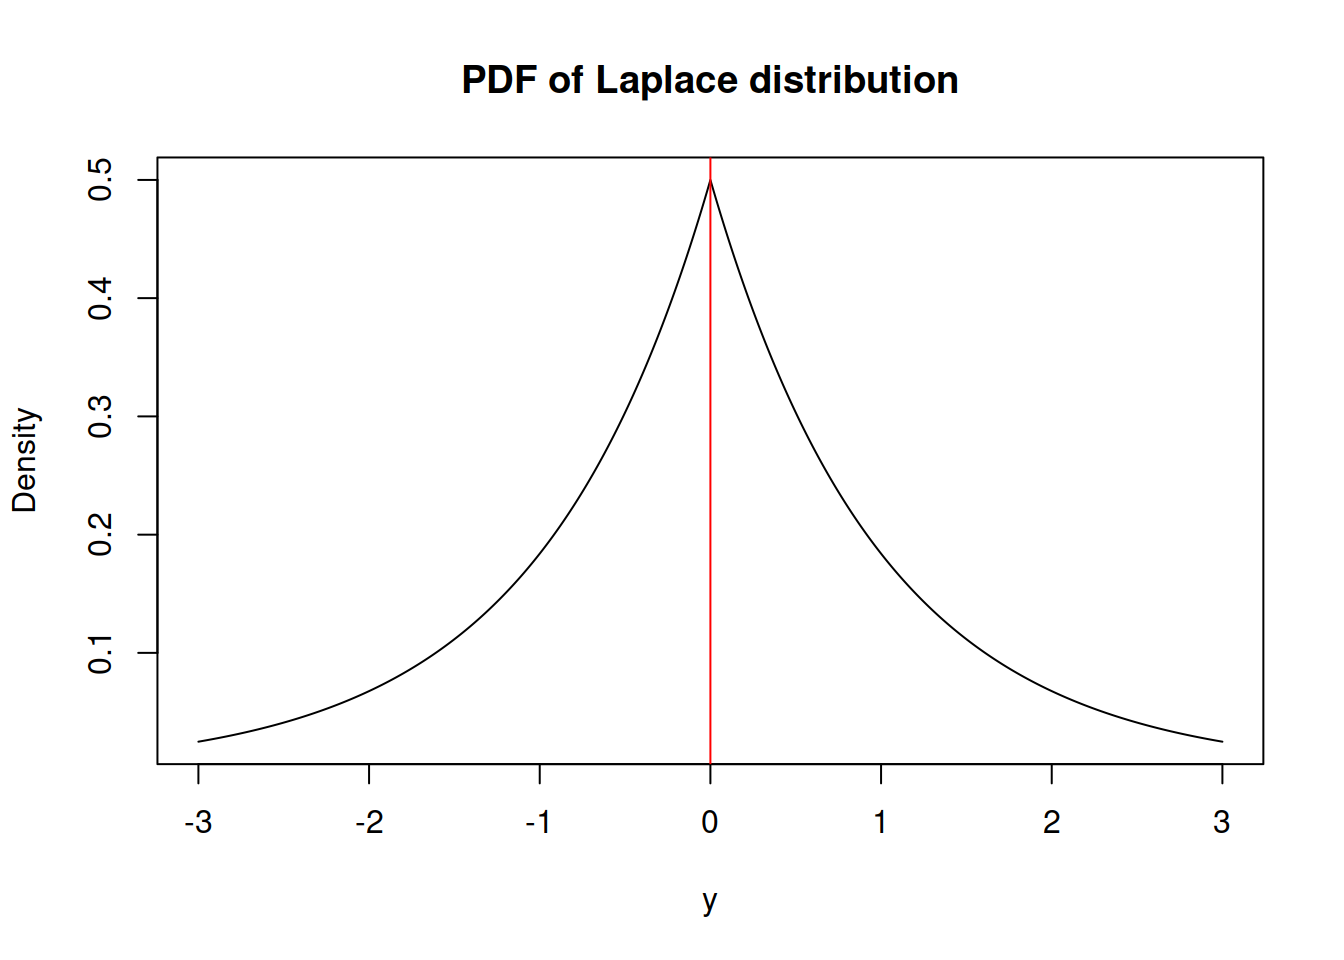
\includegraphics{adam_files/figure-latex/dlaplacePlot-1.pdf}

Similar to the normal distribution, the skewnes of Laplace is equal to zero. However, it has fatter tails - its kurtosis is equal to 6 instead of 3.

\hypertarget{s-distribution}{%
\subsection{S distribution}\label{s-distribution}}

This is something relatively new, but not groun braking. I have derived S distribution few years ago, but have never written a paper on that. It has the following density function:
\begin{equation} \label{eq:S}
    f(y_t) = \frac{1}{4 s^2} \exp \left( -\frac{\sqrt{|y_t - \mu_t|}}{s} \right) ,
\end{equation}
where \(s\) is the scale parameter. If estimated via maximum likelihood, the scale parameter is equal to:
\begin{equation} \label{eq:sS}
    \hat{s} = \frac{1}{2T} \sum_{t=1}^T \sqrt{\left| y_t - \mu_t \right|} ,
\end{equation}
which corresponds to the minimisation of a half of ``Mean Root Absolute Error'' or ``Half Absolute Moment'' (HAM). This is a more exotic type of scale, but the main benefit of this distribution is sever heavy tails - it has kurtosis of 25.2. It might be useful in cases of randomly occurring incidents and extreme values (Black Swans?).

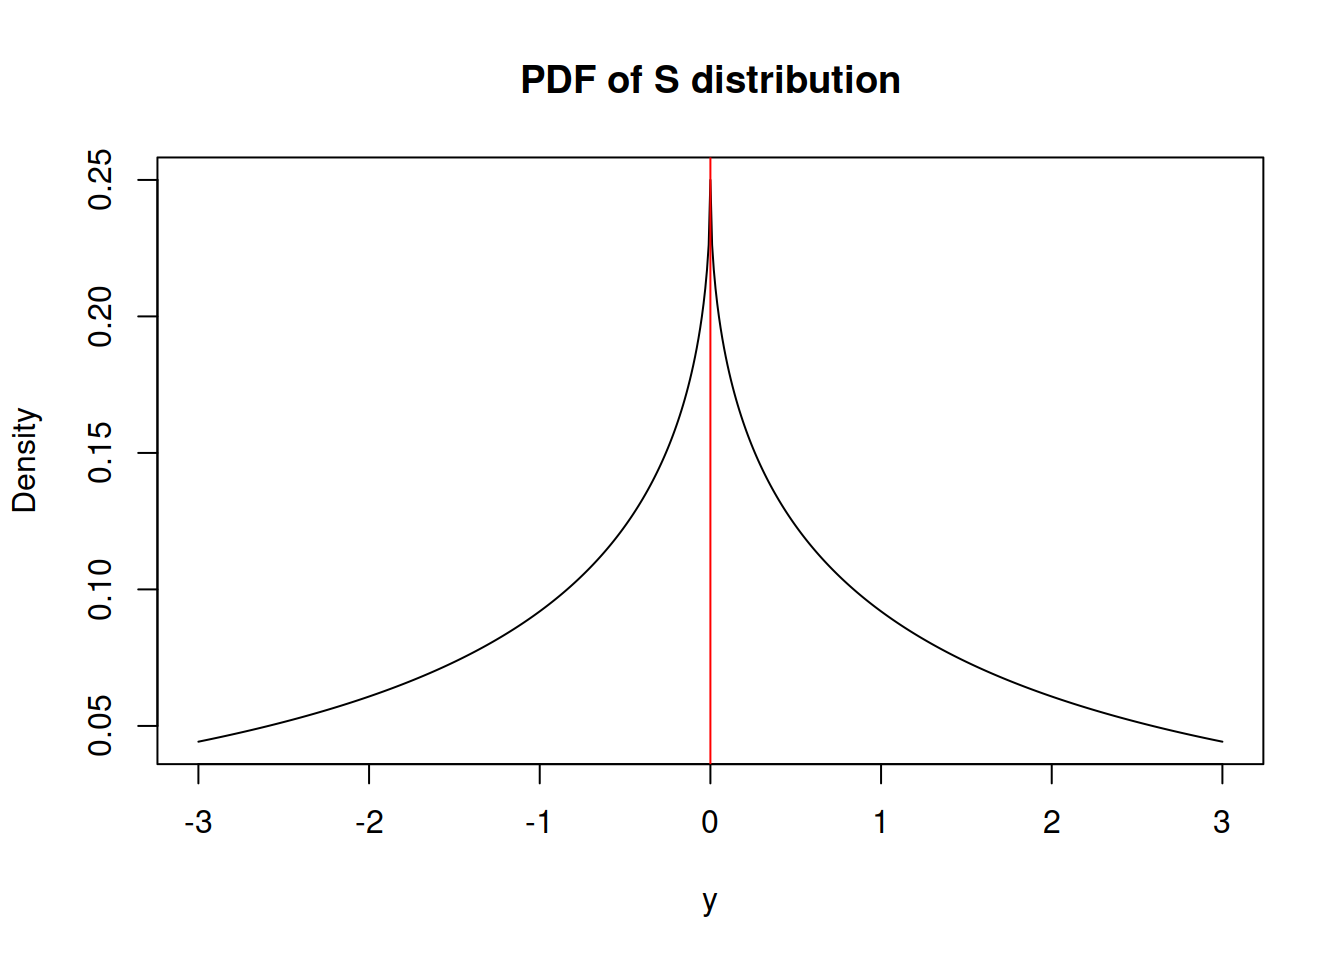
\includegraphics{adam_files/figure-latex/dsPlot-1.pdf}

\hypertarget{generalised-normal-distribution}{%
\subsection{Generalised normal distribution}\label{generalised-normal-distribution}}

Generalised normal distribution (as the name says) is a generalisation for normal distribution, which also includes Laplace and S as special cases. There are two versions of this distribution, we are mainly interested in the first one, which has the following PDF:
\begin{equation} \label{eq:GND}
    f(y_t) = \frac{\beta}{2 s^{\beta^{-1}} \Gamma(\beta^{-1})} \exp \left( -\frac{|y_t - \mu_t|^{\beta}}{s} \right),
\end{equation}
where \(\beta\) is the shape parameter, and \(s\) is the scale of the distribution, which, when estimated via MLE, is equal to:
\begin{equation} \label{eq:sGND}
    \hat{s} = \frac{\beta}{T} \sum_{t=1}^T\left| y_t - \mu_t \right|^{\beta} ,
\end{equation}
which has MSE, MAE and HAM as special cases, when \(\beta\) is equal to 2, 1 and 0.5 respectively. The parameter \(\beta\) influences the kurtosis directly, it can be calculated for each special case as \(\frac{\Gamma(5/\beta)\Gamma(1/\beta)}{\Gamma(3/\beta)^2}\). The higher \(\beta\) is, the lower the kurtosis is.

The advantage of GN distribution is it's flexibility. In theory, it is possible to model extremely rare events with this distribution, if the shape parameter \(\beta\) is fractional and close to zero. Alternatively, when \(\beta \rightarrow \infty\), the distribution converges pointwise to the uniform distribution on \((\mu_t - \sqrt[^\beta]{s}, \mu_t + \sqrt[^\beta]{s})\).

Note that the estimation of \(\beta\) is a difficult task, especially, when it is less than 2 - the MLE of it loose properties of consistency and asymptotic normality.

\hypertarget{methods}{%
\chapter{Methods}\label{methods}}

We describe our methods in this chapter.

\hypertarget{applications}{%
\chapter{Applications}\label{applications}}

Some \emph{significant} applications are demonstrated in this chapter.

\hypertarget{example-one}{%
\section{Example one}\label{example-one}}

\hypertarget{example-two}{%
\section{Example two}\label{example-two}}

\hypertarget{final-words}{%
\chapter{Final Words}\label{final-words}}

We have finished a nice book.

\bibliography{library.bib,packages.bib}

\end{document}
